\documentclass[a4paper,10pt]{report}

\usepackage[utf8]{inputenc}
\usepackage[T1]{fontenc}
\usepackage{lmodern}
\usepackage{amsmath}
\usepackage{amssymb}
\usepackage{amsthm}
\usepackage{textcomp}
\usepackage{wasysym}
\usepackage[top=2cm, bottom=2cm, left=2.1cm, right=2.1cm]{geometry}
\usepackage{fancyhdr}
\usepackage{graphicx}
\usepackage[svgnames,table]{xcolor}
\usepackage{tikzsymbols}
\usepackage{longtable}
\usepackage{listings}
\usepackage{eurosym}
\usepackage{float}
\usepackage{enumerate}
\usepackage{wrapfig}
\usepackage[francais]{babel}
\pagestyle{fancy}

\theoremstyle{remark}
\newtheorem*{rem}{\textcolor{Teal}{Remarque}}

\newcommand\R{\mathbf{R}}
\newcommand\N{\mathbf{N}}
\newcommand\C{\mathbf{C}}
\newcommand\Q{\mathbf{Q}}
\newcommand\Z{\mathbf{Z}}
\newcommand\E{\mathcal{E}}
\newcommand{\abs}[1]{\left\lvert#1\right\rvert}

\newcommand\leaf{\textcolor{ForestGreen}{\textleaf}}
\newcommand\emo{\textcolor{OrangeRed}{\smiley}}

\DeclareMathOperator{\argmax}{arg\ max}
\DeclareMathOperator{\sgn}{sgn}

\newcommand{\intervalle}[4]{\mathopen{#1}#2\mathclose{}\mathpunct{};#3\mathclose{#4}}
\newcommand{\intiff}[2]{\intervalle{[\![}{#1}{#2}{]\!]}}

\newcommand\ct{\cellcolor{LimeGreen}}
\newcolumntype{M}[1]{>{\centering}m{#1}}
\newcommand\cs{\qquad \textcolor{OrangeRed}{$\bigstar$}}


\fancyhf{}
\renewcommand{\headrulewidth}{0pt}
\fancyfoot[C]{\tiny PACT 5.1 - PAN 4}
\fancyfoot[RO]{\thepage}
\fancyfoot[LE]{\thepage}

\usepackage[colorlinks=true,linkcolor=purple]{hyperref}


\begin{document}


%%%%%%%%%%%%%%%%%
% Page de titre %
%%%%%%%%%%%%%%%%%


\begin{titlepage}
	\newcommand{\HRule}{\rule{\linewidth}{0.5mm}}

	\center

	\textsc{\LARGE Télécom ParisTech}\\[1.2cm]
	\textsc{\Large PACT 2016-2017}\\[0.5cm]

	\HRule \\[0.8cm]
	{ \huge \bfseries Rapport d'avancement du groupe 5.1}\\[0.4cm]
	{ \huge \bfseries Projet FeelList}\\[0.4cm]
	\HRule \\[1.5cm]

	\begin{minipage}{0.4\textwidth}
	\begin{flushleft} \large
	\emph{Groupe :}\\
	Charles \textsc{Boulitrop}\\
	Grégoire \textsc{Dupont}\\
	Philippe \textsc{Edwards}\\
	Ilyass \textsc{El Mansouri}\\
	Régis \textsc{Gourdel} \\
	Nesrine \textsc{Kortas}\\
	Annah \textsc{Tencic}\\
	\end{flushleft}
	\end{minipage}
	~
	\begin{minipage}{0.4\textwidth}
	\begin{flushright} \large
	\emph{Tuteurs :} \\
	Prénom \textsc{Nom}\\
	Prénom \textsc{Nom}\\
	\vspace{1em}
	\emph{Encadrant génie logiciel :}\\
	Prénom \textsc{Nom} \\
	\end{flushright}
	\end{minipage}\\[1.3cm]

	{\large \today}\\[0.9cm]

	% À commenter au PAN 1 car pas encore utile
	% La coloration pour les parties nouvelles devra ensuite se faire de la même manière que pour le mot bleue ci-dessous
	\begin{rem}
		Pour le PAN 4 les ajouts et modifications ont été signalés par la couleur \textcolor{RoyalBlue}{bleue}.
		Lorsque le titre d'une section est coloré c'est que l'ensemble du contenu est concerné.\\[0.9cm]
	\end{rem}

	\begin{figure}[htp]
	\centering
	
\includegraphics[scale=0.60]{./images/logoPACT.jpg}
	\end{figure}

	\begin{figure}[htp]
	\centering
	
\includegraphics[scale=0.12]{./images/logoTelecom.png}
	\end{figure}

\end{titlepage}


\newpage

\tableofcontents

\newpage

%%%%%%%%%%%%%%%%%%%%%%%%
% Sections principales %
%%%%%%%%%%%%%%%%%%%%%%%%

\chapter{Résumé du projet}
	\section{Résumé du sujet choisi en français}

	Notre projet consiste en l’élaboration d’une application exclusivement utilisable sur ordinateur qui propose à l’utilisateur une liste de lecture musicale adaptée à ses goûts mais aussi à son humeur du moment.
	Nous l’avons baptisé FeelList.
		
	Le fonctionnement de l’application est assez simple.
	De prime abord l’ordinateur prend une photo de l’utilisateur afin d’en extraire des traits du visage caractéristiques d’une certaine humeur.
	Après la détermination de l’humeur, l’application propose à l’utilisateur une liste de lecture composée de morceaux extraits de sa bibliothèque personnelle mais aussi d’une bibliothèque par défaut que nous aurons rendue publique sur un cloud.
	En plus de faire gagner du temps à l’utilisateur - qui ne sait pas choisir parmi les nombreuses pistes audio de sa bibliothèque - FeelList a aussi la qualité de faire découvrir de nouveaux morceaux à ce dernier.

	Cependant une question majeure se pose : quelle type de musique écouter dans telle ou telle situation ?
	En effet le choix d’un morceau adapté à une humeur est éminemment individuel et subjectif.
	C’est pour cela que nous permettons à l’utilisateur de choisir.
	Lors de la configuration initiale, l’application propose à l’utilisateur d’indiquer dans quelle humeur il souhaiterait écouter tel ou tel morceau extrait de sa bibliothèque personnelle.
	Le détail de cet étiquetage est présenté plus loin dans ce rapport.

	Ce projet s’inscrit parfaitement dans le thème « du geste au son ».
	En effet, à partir d’une photo nette de l’utilisateur, l’application propose une traduction musicale de certaines modalités du visage.
	Autrement dit, elle passe du geste au son.

\section{English summary}

	Our project is to build a computer application that suggests a musical playlist adapted to the user’s tastes and to their mood.
	We decided to name it FeelList.
		
	The way it goes is quite simple.
	The application starts off by taking a picture of the user in order to extract from it relevant signs of a prominent mood.
	Once FeelList has managed to determine the user’s mood it delivers a musical playlist containing tunes from his personal library but also some from a public library that would have been put on a cloud beforehand.
	In a nutshell, FeelList isn’t only a huge timesaver for people that don’t know what to listen to, it also helps users discover new authors and albums.
		
	However not everyone agrees on the type of music you want to listen to once you’re in a certain mood.
	The choice of listening to a particular type of music when you’re in a special mood is unmistakably personal and subjective.
	FeelList therefore offers such a choice.
	The first time you download the app, you have to fill in a grid in which you indicate in which mood you would like to listen a large choice of tunes from your own library.

	Our project fits in perfectly with the yearly theme : « turn movements into sounds » as it evidently associates musical playlists with face motions that transcript moods and emotions.


\chapter{Étude d’antériorité et justification de la proposition}

	\section{Description de la proposition}
		Nous proposons la création d’une application capable de lier des données visuelles à des informations résultantes portant sur la musique et les goûts musicaux.
Les données en questions sont des photos de visages prises de l’utilisateur dans un état d’âme bien spécifique, le résultat en question est une playlist adapté à son humeur du moment.\\

L’application s’adresse à un public amateur de musique et plus particulièrement au public avec un nombre important de musiques dans son répertoire en leur suggérant des morceaux adaptés à son humeur.
Il peut également viser un public recherchant des musiques similaire à ce qu’il écoute, grâce aux recommandations que propose l’application.

\begin{figure}[htp]
	\centering
	
\includegraphics[scale=3.00]{images/logo2.png}
	\caption{Logo de l'application}
\end{figure}
		
	\section{Description du pourquoi}
		L’idée de base du projet a énormément évolué pour devenir ce qu’elle est actuellement.
En effet, l’idée d’origine était de réaliser une application capable de traduire le langage des signes en phrases cohérentes.
Mais durant la foire aux experts il est apparu que la traduction du LSF en phrases cohérentes est irréalisable : on ne peut pas utiliser une Kinect pour une telle précision sur les mouvements des doigts et Leapmotion (carré de 50cm avec ondes radio reconnaissant les mouvements d’une main) n’est pas approprié (2 mains à gérer implique de relier des plaques entre elles, sans oublier de les relier aussi à la reconnaissance émotionnelle, ce qui est infaisable pour nous; il faut être statique et l’amplitude des mouvements est limitée, c’est pourquoi le Leapmotion ne convient que pour commander une souris virtuelle devant son ordinateur).
Ainsi la solution était de se concentrer uniquement sur les émotions/humeurs/états.
Le passage de l’émotion à un morceau de musique nous a semblé pertinent, en effet la reconnaissance multimodales d’émotions dans des applications interactives est un modèle jeune dont la maturité est grandissante et de plus en plus de chercheurs travaillent sur ce domaine pour améliorer l’interaction homme-machine, et de plus en plus d’applications innovantes utilisant les modèles de la théorie de l’émotion sont entrain d’apparaître dans le marché.\\

Néanmoins, nous avons du faire face à plusieurs obstacles pour concrétiser ce projet.

Tout d’abord, en ce qui concernent l’interprétation du visage pour les associer à des émotions, nous travaillerons sur les états : triste, joyeux, en colère.
Ces états sont plus facilement reconnaissables sans ambiguïté: l'état triste se manifestera par une inertie des mouvements au contraire de l'état heureux/joyeux où il y aura profusion de petits mouvements (hochement de tête, changements rapides et multiples de mimiques...).
L'état heureux sera surtout visible au sourire et au plissement des yeux au contraire de l'état triste.
Ce type de paramètres nous semble déjà plus pertinent et moins controversé, et nous approfondirons cette recherche des attributs adéquats dans le module reconnaissance d’émotion, où on dégagera des paramètres de classement pertinents, invariants et différenciant.

Ainsi notre application répondra à un besoin, qu’on retrouve souvent chez de nombreux utilisateurs, en effet l’idée est apparu pertinente quand en discutant avec des camarades ou des collègues on se rend compte que nous ne sommes pas les seuls à avoir du mal à sélectionner les morceaux que l’on souhaite écouter.
De plus la reconnaissance d’émotion est un domaine jeune qui risque très probablement par la loi de Say selon laquelle « l’offre crée sa propre demande », d’attirer de nombreux utilisateurs.

\textcolor{RoyalBlue}{
Notre application se distingue des produits préexistants sur plusieurs points.
Par rapport à une utilisation où l'utilisateur choisit “manuellement” les musiques qu'il souhaite écouter : il y a ici un gain de temps pour lui, il aura juste à passer un moment pour \textit{tagger} une partie de ses musiques au début, des tags sur les musiques restantes seront extrapolées par classification et l'utilisateur aura juste à lancer le mode spécifique FeelList.
Par rapport à un service qui propose des playlists classées par humeur : FeelList a l'avantage de la personnalisation, si l'humeur influe sur ce que l'on écoute, tout le monde n'écoute pas pour autant les mêmes musiques dans la même humeur.
}
		
	\section{Description de l’état de l’art}
		Comme nous l’avons expliqué précédemment, la reconnaissance d’émotions est un domaine jeune mais dont la maturité grandissante impliquera des applications diverses, ainsi on retrouve des applications tel que Picxel qui a développé un kit logiciel qui identifie les émotions du visage lorsque l'utilisateur est devant son ordinateur, permettant à la machine de s'adapter en conséquence.

\begin{figure}[htp]
\centering
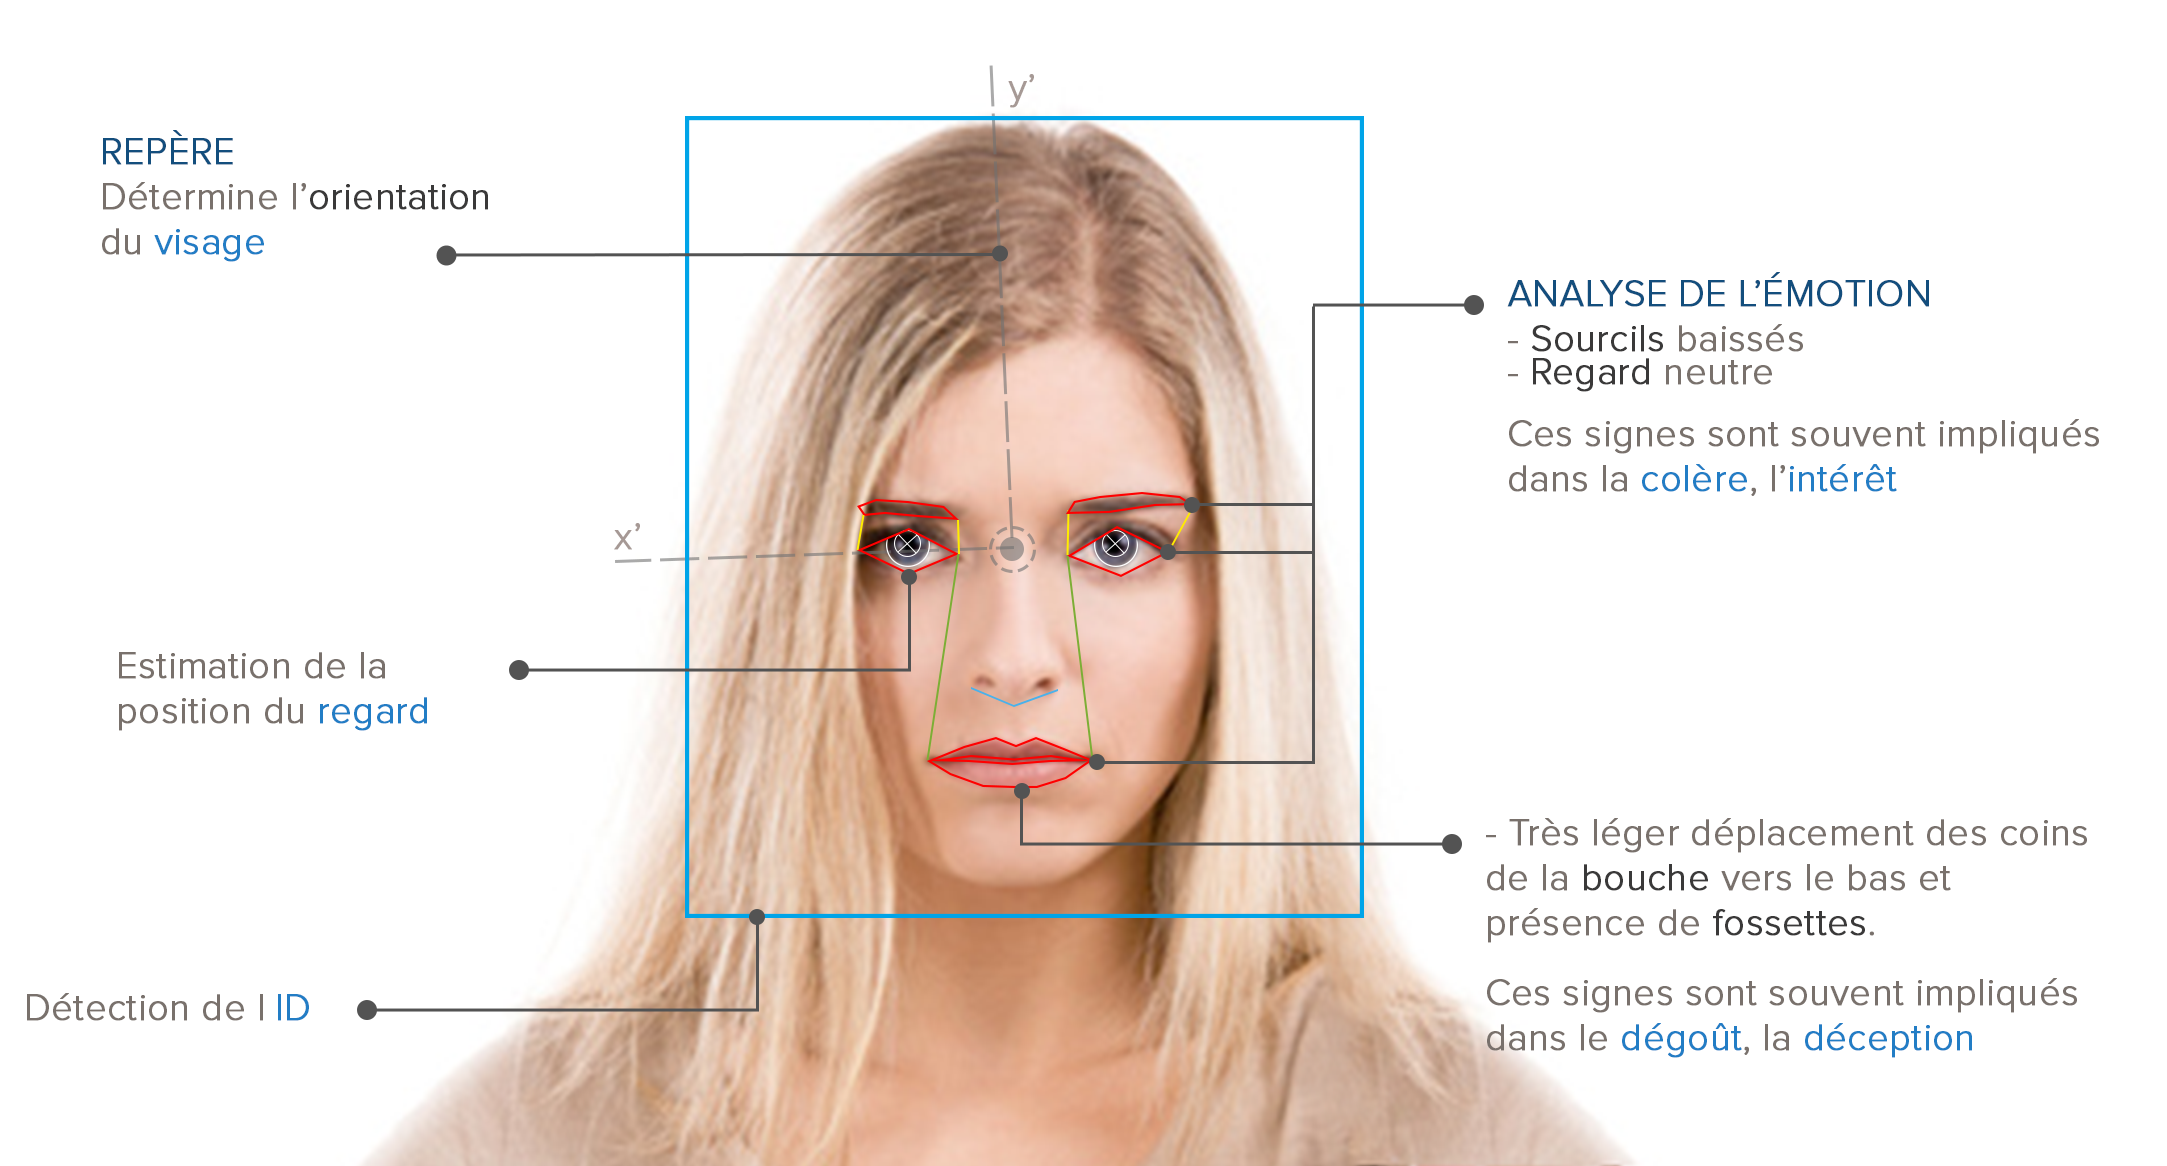
\includegraphics[scale=0.9]{./images/etatArt1.png}
\caption{Image issue de picxel.fr - Illustration de la colère}
\label{eA1}
\end{figure}

On retrouve également la société Beyond Verbal qui a lancé une application qui permet d’extraire, de décoder et de mesurer un spectre d’émotion à partir de la voix brute d’une personne.
Ou encore une application pour Google Glass baptisée Emotient qui permettra à l’utilisateur d’obtenir des informations sur les émotions de son interlocuteur.\\

Par ailleurs, la classification de l’émotion générée par la musique n’est pas quelque chose de nouveau, en effet on retrouve des services web tel que Musicovery qui effectue une classification des musiques sur un repère orthogonal avec deux axes : calme-énergétique et sombre-positif (Cf figure \ref{eA2}).

\begin{figure}[htp]
\centering
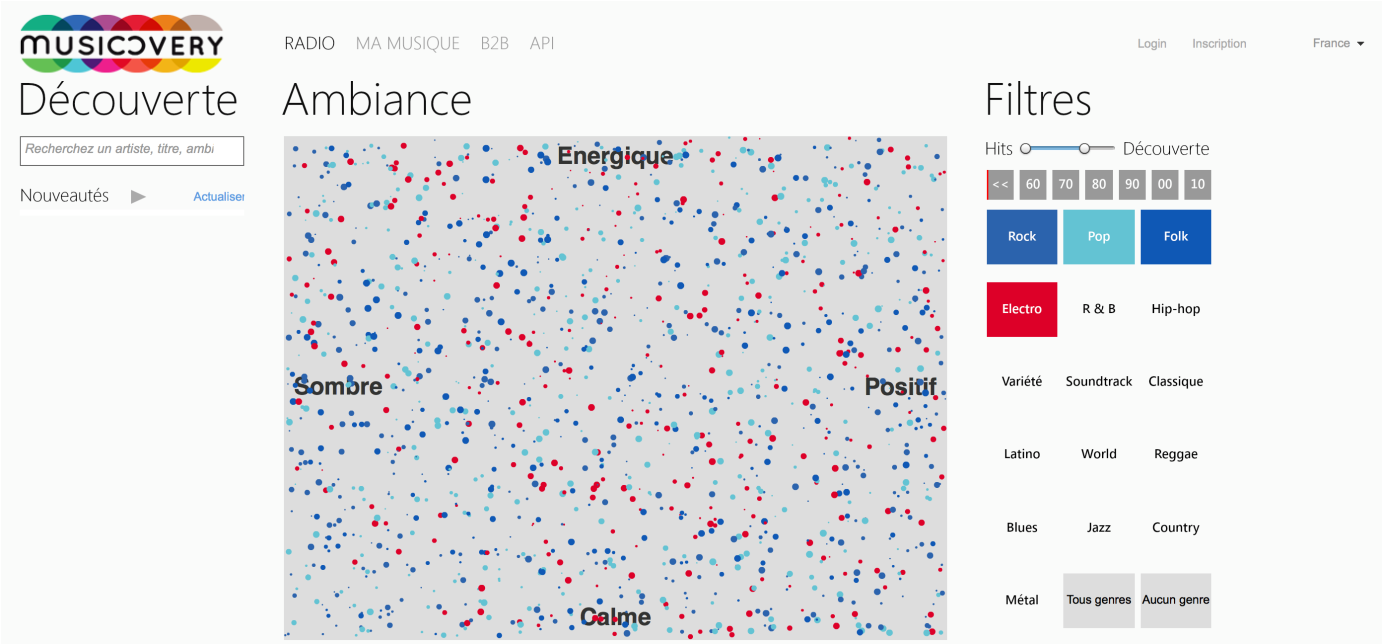
\includegraphics[scale=1.0]{./images/etatArt2.png}
\caption{Capture d'écran du site de streaming Musicovery}
\label{eA2}
\end{figure}

Dans un genre proche, certains sites de streaming ou applications tels que \emph{Stereomood} ou \emph{Moodflow} permettent d'accéder à une playlist correspondant à une émotion.
Cependant, dans ce cas c'est à l'utilisateur de choisir la playlist qu'il doit écouter, en cherchant donc dans un premier temps à identifier sa propre émotion.
De plus les musiques proposées par ces deux services sont celles d'une certaine base de musiques sur internet, et pas les musiques de l'utilisateur.

De même, l'analyse des goûts musicaux à partir de playlists, à travers une classification automatique se retrouve dans certains projets récents tel que \textit{Prizm}, lancé par une startup française et dont la commercialisation doit commencer début 2016.
C'est un objet diffusant de la musique choisie automatiquement, en fonction des goûts des utilisateurs et de l'ambiance de la pièce où il se trouve.
De plus il devient de plus en plus “intelligent” à mesure qu'on interagit avec lui.
Cela fournit un exemple de recommandation en fonction de paramètres extérieurs, et non juste selon un filtrage collaboratif, auquel sont limités les sites de streaming.
Ainsi ce processus de machine learning pourra également être utilisé dans le cadre de la classification automatique de nos musiques.

\begin{figure}[htp]
\centering
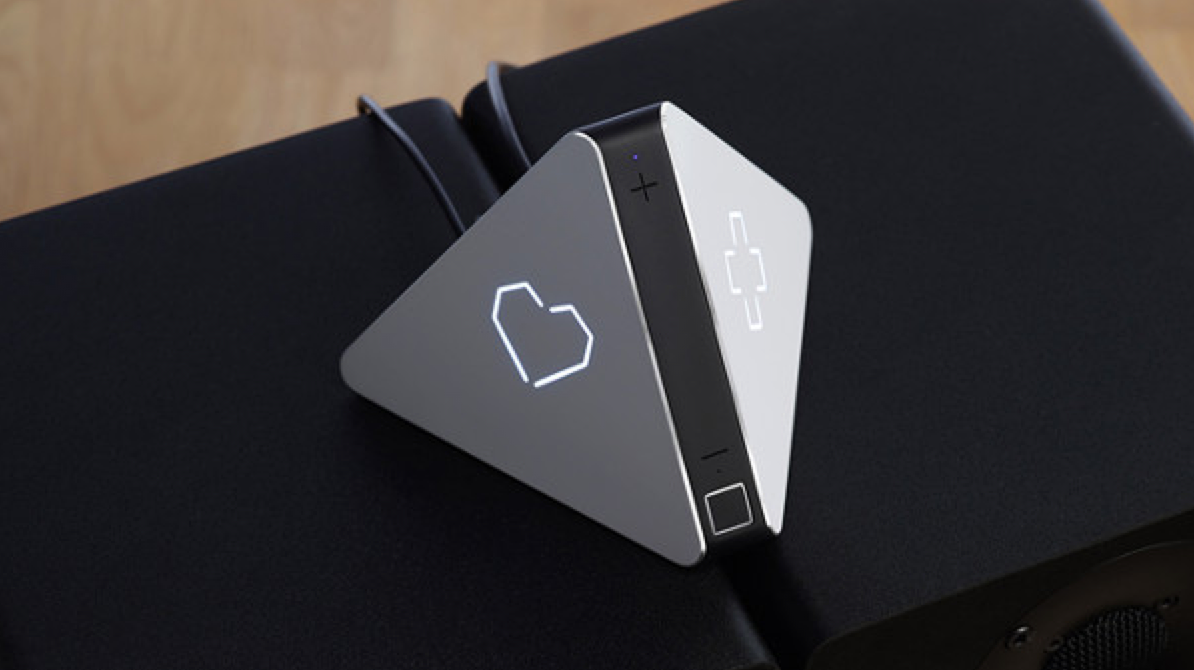
\includegraphics[scale=0.70]{./images/etatArt3.png}
\caption{Boîtier de Prizm}
\end{figure}

Il restera donc, dans le cadre de notre projet, à construire ce « pont » qui nous permettra de relier l’émotion ressentie par l’utilisateur et l’ambiance suscitée par la musique, ce qui marquera le côté innovant de notre projet.



\chapter{Scénarios d’usage}

	\setlength{\fboxsep}{3.4mm}

\begin{wrapfigure}{r}{0.35\textwidth}
	\fbox{
	\begin{minipage}[c]{5cm}
		\emph{Matériel :}
		\begin{itemize}
			\item Ordinateur : PC ou Mac.
			\item Webcam : intégrée à l'ordinateur ou clipsable et reliée à l'ordinateur.
		\end{itemize}
	\end{minipage}
	}
\end{wrapfigure}

Pierre adore écouter de la musique, si bien qu’il possède quelques centaines de musiques dans son répertoire de morceaux sur son ordinateur.
Cependant, il lui arrive parfois de ne pas savoir quel morceau écouter, du fait de cette trop grande diversité.
Un jour, alors qu’il a invité son ami Paul chez lui, ce dernier est surpris de voir Pierre passer de longues minutes à choisir le morceau qu’ils vont écouter, puis s'irrite de le voir systématiquement interrompre chaque morceau qui a l'air prometteur au bout de quelques secondes pour en proposer un autre.
Paul conseille donc à Pierre de télécharger l’application FeelList pour lui faire gagner du temps dans sa recherche de la musique la plus adéquate.

Cette application suit un principe simple : à partir de très courtes vidéos du visage de l’utilisateur, l'application identifie son expression et l'associe à un état ou une émotion (joie, tristesse, agacement, fatigue...), puis lui propose une liste de morceaux en adéquation avec son humeur et ses goûts musicaux.
Elle a pour vocation d'être à la fois une aide au choix personnalisée et un moyen de découverte musicale pour des utilisateurs assez statiques positionnés devant la webcam.
C'est exactement ce qu'il lui faut !

Pierre décide alors de télécharger l’application et de l’essayer tout de suite.\\

\begin{wrapfigure}{l}{0.42\textwidth}
	\fbox{
	\begin{minipage}[c]{6cm}
		\emph{Installation et initialisation de FeelList sur PC/Mac :}
		\begin{itemize}
			\item L'utilisateur crée un profil avec son nom d’utilisateur, une photo neutre de son visage.
			\item Il coche, parmi une liste générique, les styles de musique qu’il préfère (rock, rap, RnB,...).
		\end{itemize}
	\end{minipage}
	}
\end{wrapfigure}

Il se place devant la webcam de son ordinateur.
L’application prend à intervalle régulier de très courtes vidéos et détecte son expression (joyeuse car son ami est chez lui).
Puis, elle se connecte via internet à la banque son par défaut FeelList qui se trouve sur le \textit{cloud}.
Les morceaux de cette banque par défaut ont été arbitrairement répartis par catégories d' « émotions »  et classées par styles.
L'application sélectionne et propose alors une liste de musiques joyeuses correspondant à l'état d'esprit de Pierre et respectant les critères de style musical qu'il a choisis lors de la création de son profil.
Pierre est enchanté de ces propositions, d'autant plus qu'elles lui permettent de découvrir de nouveaux morceaux !\\

\begin{wrapfigure}{r}{0.55\textwidth}
	\fbox{
	\begin{minipage}[c]{7.6cm}
		\emph{Intégration de morceaux de son propre répertoire musical aux propositions de FeelList :}
		\begin{itemize}
			\item L'utilisateur se connecte sur son profil.
			\item Il importe son répertoire musical.
			\item Il classe tous ou une partie de ses morceaux en les taggant : à côté de chaque titre se trouvent différents smileys cliquables (parmi lesquelles « \textit{Angry} », « \textit{Tired} », « \textit{Happy} »...).
		\end{itemize}
	\end{minipage}
	}
\end{wrapfigure}

Dans la semaine, alors que Pierre travaille sur son ordinateur, il décide de réutiliser l'application pour travailler en musique.
Cependant, il voudrait pouvoir écouter aussi les morceaux figurant dans son propre répertoire en plus de ceux de la banque son par défaut.
À son agréable surprise, il découvre que c'est possible.

Par exemple, il appose le smiley « \textit{Angry} » aux morceaux qu'il aime écouter lorsqu'il est agacé, qu'ils soient tranquilles pour l'apaiser ou au contraire forts et expressifs pour l'aider à évacuer sa colère, en fonction de ce qu'il préfère écouter selon son humeur.
Ensuite, tout au long de sa soirée de travail, l'application prend de courtes vidéos du visage de Pierre à intervalles réguliers pour cerner son humeur, et lui propose d'écouter un panel de morceaux issus pour certains de son propre répertoire, les autres venant de la banque par défaut.
Les propositions évoluent avec ses changements prolongés d'humeur.

Cependant, si Pierre n'étiquette aucun morceau ou pas assez, FeelList ne proposera que des morceaux issus de la banque par défaut.
De plus, si Pierre n'est pas connecté à internet, il n'aura accès qu'au « mode hors ligne » de l'application, c'est-à-dire que les morceaux proposés ne seront issus que de son propre répertoire.
S'il n'a ni étiqueté de morceaux, ni de connexion internet, l'application ne fonctionne pas en mode détection des émotions et il sera obligé de lancer des musiques “à la main” comme sur un lecteur classique.\\

\begin{wrapfigure}{l}{0.42\textwidth}
	\fbox{
	\begin{minipage}[c]{6cm}
		\emph{Option film :}
		\begin{itemize}
			\item Ils clipsent une petite caméra au-dessus de l'écran plat de Jacques.
			\item Ils la relient à l'ordinateur.
			\item Jacques se connecte sur son profil (qu'il vient de créer).
			\item Il clique sur « Option film » et entre sa durée.
			\item Il augmente la luminosité dans la pièce si FeelList lui affiche un message signalant qu'elle ne peut pas procéder à la détection du visage et l'analyse des émotions dans la pénombre.
		\end{itemize}
	\end{minipage}
	}
\end{wrapfigure}

Deux mois plus tard Pierre et Paul sont invités à aller voir un film chez Jacques, un autre de leurs amis, à l'occasion de l'anniversaire de ce dernier.
Ils projettent ensuite de passer la fin de la soirée ensemble, et en musique. Pierre et Paul parlent alors de FeelList à Jacques qui semble tout de suite intéressée par le concept.

L'application détecte le visage de Jacques et se focalise sur uniquement sur celui-ci en ignorant Pierre et Paul, puisque c'est le profil de Jacques qui est utilisé.
Elle est programmée pour se mettre en route et débuter la prise de photos à intervalles réguliers et leur analyse 10 minutes avant la fin du film.
Cependant, ils interrompent le film à plusieurs reprises car Jacques reçoit de nombreux coups de fils pour son anniversaire : FeelList en prend compte, car elle détecte quand l’utilisateur n’est plus dans son champ de vision et décale sa mise en route de la durée des absences de Jacques.

Les trois amis sont très émus par la fin du film, et l'application leur propose une série de morceaux, issus à la fois du répertoire de Jacques et de la banque son par défaut, en accord avec l'expression relativement attristée de Jacques et ses goûts musicaux.
Pierre, Paul et Jacques passent alors une très bonne soirée, satisfaits d’avoir pu garder l’atmosphère du film bien qu’il soit fini, les propositions évoluant ensuite avec l'enthousiasme croissant de Jacques qui reste assis devant la caméra à bavarder joyeusement avec ses amis.

\chapter{Architecture du projet}

	\section{Schéma d’architecture}
		Voir figure \ref{diagArchi}.

		\begin{figure}[htp]
		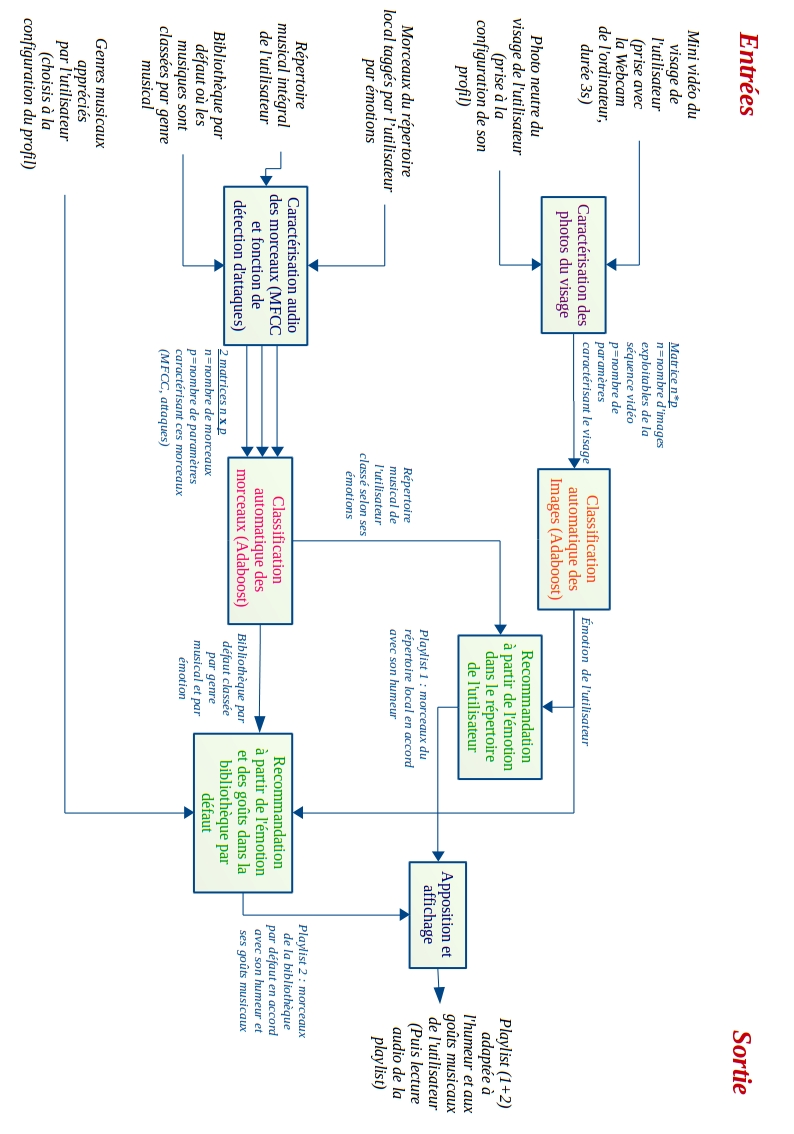
\includegraphics[scale=0.60]{images/diagrammeArchitecture.jpg}
		\caption{Diagramme d'architecture du projet}
		\label{diagArchi}
		\end{figure}

	\section{Description des blocs}
		\subsection{Traitement de l’image}
\label{dB1}

	\subsubsection{Les entrées}
	\label{dB1.1}

		\begin{enumerate}[(i)]
		\item De prime abord, lors de la configuration initiale de l’application, l’utilisateur devra prendre une (ou plusieurs) \emph{photo(s) « neutre(s) »} de son visage qui servira d’outil(s) comparatif(s) pour la reconnaissance des humeurs lors de l’utilisation courante de l’application.
		\item Lors de cette utilisation courante, l’ordinateur prendra une vidéo du visage de l’utilisateur qui présentera une humeur particulière.
		\end{enumerate}

	\subsubsection{Caractérisation des photos du visage}
	\label{dB1.2}

		\begin{enumerate}[(i)]
		\item Le traitement de l’image prise au cours de l’utilisation courante consiste principalement à y dégager $p$ caractéristiques renvoyant à une humeur particulière.
		\item Pour chaque photo exploitable de la vidéo on extrait $p$ paramètres caractérisant le visage.
		\end{enumerate}

	\subsubsection{Classification automatique des images}
	\label{dB1.3}

		On classe les $n$ photos extraites de la vidéo en fonction des $p$ caractéristiques.

\subsection{Traitement audio}
\label{dB2}

	\subsubsection{Les entrées}
	\label{dB2.1}

		\begin{enumerate}[(i)]
		\item Lors de la configuration initiale l’application demandera à l’utilisateur d’attribuer à un échantillon de musiques de son répertoire l’humeur dans laquelle il aime écouter tel ou tel morceau.
			On appellera cette opération le \emph{taggage} (ou \emph{étiquetage}) des morceaux.
		\item L’application disposera par ailleurs de l’intégralité de son répertoire musical ainsi qu’une bibliothèque « par défaut » que les créateurs de l’application auront mis à disposition de l’utilisateur.
		\end{enumerate}

	\subsubsection{Caractérisation audio des morceaux}
	\label{dB2.2}

		Le traitement audio consiste en l’analyse des grandeurs intrinsèques sonores d’une chanson par exemple de son tempo, de sa modalité (majeure ou mineure) ou encore de son MFCC.
		De nouveau, il s’agira d’attribuer aux $n$ morceaux les $p$ caractéristiques intrinsèques.

	\subsubsection{Classification automatique}
	\label{dB2.3}

		\begin{enumerate}[(i)]
		\item C’est ici que rentre en jeu le point (i) de la section « les entrées » du \ref{dB2.1} : l’utilisateur ayant attribué à un échantillon de chansons une humeur particulière, ces chansons sont aussi caractérisés par les coordonnées définissant l’humeur ou l’état.
			\begin{rem}
			L’utilisateur pourra, durant l’utilisation courante, choisir de modifier son étiquetage initial. \emph{Une fois la mise à jour lancée par l’utilisateur}, une nouvelle classification de la musique se fera automatiquement.
			\end{rem}
		\item On compare ensuite les grandeurs intrinsèques sonores des morceaux non taggés et de ceux qui l’ont été à la configuration initiale pour déterminer automatiquement à quelles humeurs correspondent les chansons non étiquettées.
		\end{enumerate}

		Dès lors l’intégralité du répertoire de l’utilisateur, ainsi que la bibliothèque « par défaut » est classé non seulement par les grandeurs intrinsèques sonores des chansons mais aussi par l’humeur dans laquelle l’utilisateur aime écouter tel ou tel morceau.

\subsection{Intégration et comparaison des données}
\label{dB3}

	\begin{enumerate}[(i)]
	\item Il suffit alors de comparer les données du traitement audio et du traitement image afin de proposer une liste de lecture convenant à l’humeur de l’utilisateur.
	\item S’agissant du répertoire personnel de l’utilisateur, on compare les données fournies par le traitement audio et celles fournies par le traitement image pour construire une première liste de lecture (par souci de simplicité on l’appellera \emph{playlist1}).
	\item S’agissant du répertoire « par défaut » il faudra en amont le comparer avec une autre donnée fournie par l’utilisateur lors de la configuration initiale : les genres musicaux qu’il apprécie.
		Une fois cette comparaison faite, on compare ce qui reste de la liste « par défaut » avec les données fournies par le traitement image afin de proposer une deuxième liste de lecture (idem, \emph{playlist2}).
	\end{enumerate}

	On obtient donc (après apposition des deux listes de lecture) une liste de lecture finale adaptée à l’humeur de l’utilisateur.
	Cette liste est constituée non seulement de chansons connues de l’utilisateur mais en plus de nouvelles chansons qu’il va découvrir et qui ont été choisies pour convenir à ses goûts musicaux ainsi qu’à son humeur.

		
	\section{Description des interfaces}
		\begin{itemize}
	\item \textbf{Interface "caractérisation des visages" - "classification automatique des images"\\}
		Le bloc de classification pourra demander au bloc de caractérisation de lui fournir une matrice $n \times p$ d'informations caractérisant le visage de la personne, où $n$ est le nombre d'images exploitables dans une vidéo de 3s prise par la webcam, et $p$ est le nombre de caractérisant le visage.
	\item \textbf{Interface "classification automatique des images" - "intersection émotion répertoire"\\}
		Le bloc d'intersection pourra demander au bloc de caractérisation l'humeur de l'utilisateur.
		Celle-ci sera sous forme de chaîne de caractères.
	\item \textbf{Interface "classification automatique des images" - "intersection émotion - goûts musicaux - bibliothèque"\\}
		Le bloc d'intersection pourra demander au bloc de caractérisation l'humeur de l'utilisateur.
		Celle-ci sera sous forme de chaîne de caractères.
	\item \textbf{Interface "caractérisation audio des morceaux" - "classification automatique des morceaux"\\}
		Le bloc de classification automatique des morceaux pourra demander au bloc de caractérisation 3 matrices de taille $n \times p$ où $n$ est le nombre de morceaux (dans une bibliothèque convenue par le bloc de caractérisation) et $p$ est le nombre de paramètres (par exemple, le tempo serait l'un deux).
	\item \textbf{Interface "classification automatique des morceaux" - "intersection émotion répertoire"\\}
		Le bloc d'intersection pourra demander au bloc de classification de \textit{tagger} les musiques d'une bibliothèque donnée avec l'humeur adaptée au morceau.
	\item \textbf{Interface "classification automatique des morceaux" - "intersection émotion - goûts muicaux - bibliothèque"\\}
		Le bloc d'intersection pourra demander au bloc de classification de \textit{tagger} les musiques d'une bibliothèque donnée avec l'humeur adaptée au morceau.
	\item \textbf{Interface "apposition et affichage" - "intersection émotion répertoire"\\}
		Le bloc apposition et affichage peut demander au bloc d'intersection une playlist  de morceaux du répertoire de l'utilisateur à jouer.
	\item \textbf{Interface "apposition et affichage" - "intersection émotion répertoire"\\}
		Le bloc apposition et affichage peut demander au bloc d'intersection une playlist  de morceaux de la bibliothèque par défaut à jouer.
\end{itemize}
		
	\section{Diagramme de séquence}
		Les modifications apportées par notre projet vont intervenir notamment au travers des trois tâches suivantes : écoute en mode FeelList, ajout d'une musique à la bibliothèque et mise à jour des données concernant cette bibliothèque, avec étiquetage automatique des morceaux non étiquetés par l'utilisateur.
On donne donc pour chacun d'eux un séquençage temporel des actions effectuées : voir figures \ref{ds1}, \ref{ds2} et \ref{ds3}.

\begin{figure}[htp]
\centering
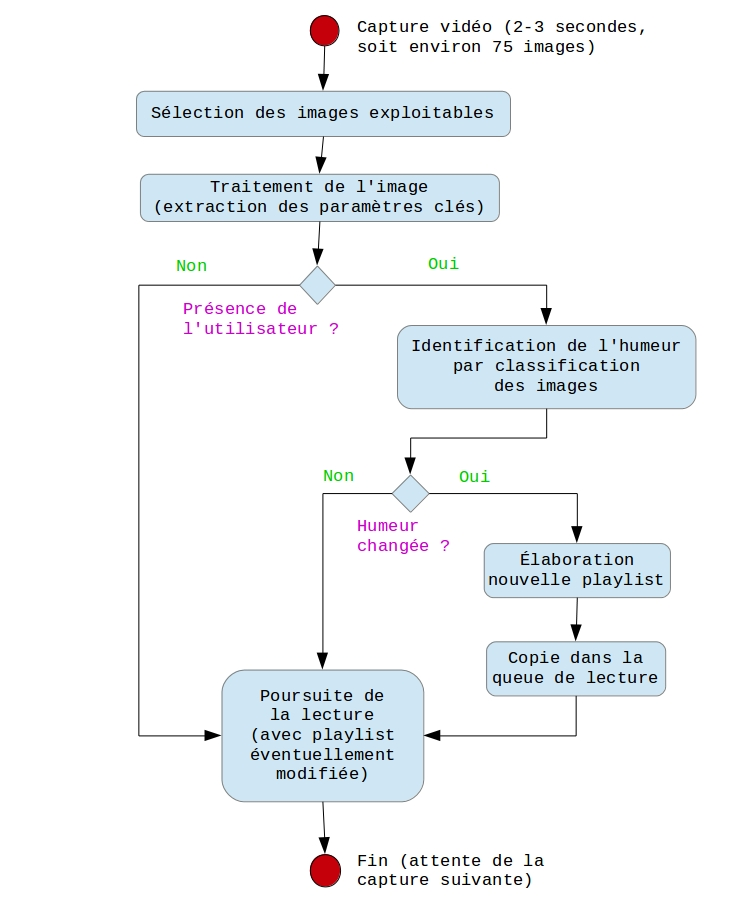
\includegraphics[scale=0.5]{./images/SchemaCaptureVideo2.jpg}
\caption{Opérations effectuées lors d'une capture vidéo par le logiciel dans le cadre d'une utilisation en mode FeelList}
\label{ds1}
\end{figure}

\begin{figure}[htp]
\centering
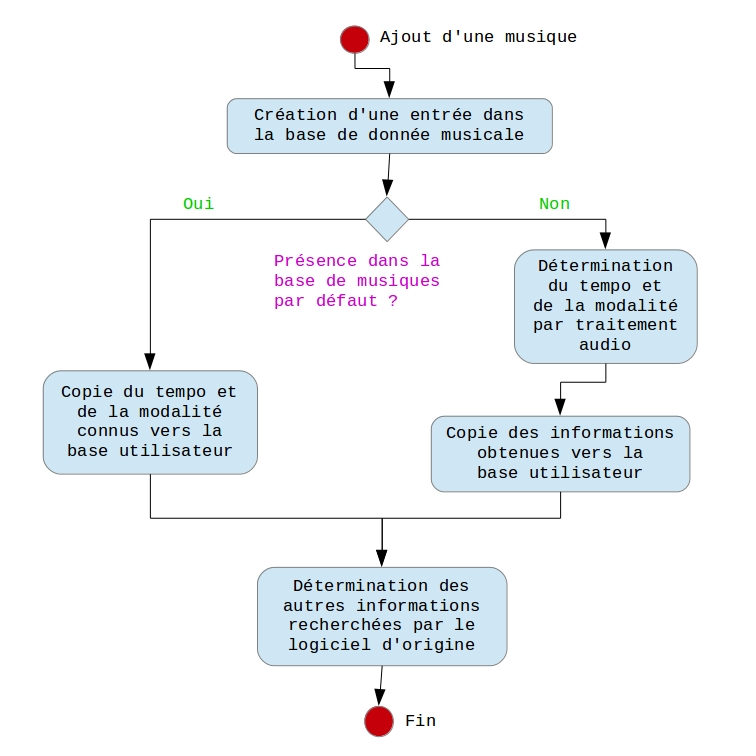
\includegraphics[scale=0.5]{./images/SchemaAjoutMusique2.jpg}
\caption{Opérations effectuées lors de l'ajout d'une musique à la bibliothèque}
\label{ds2}
\end{figure}

\begin{figure}[htp]
\centering
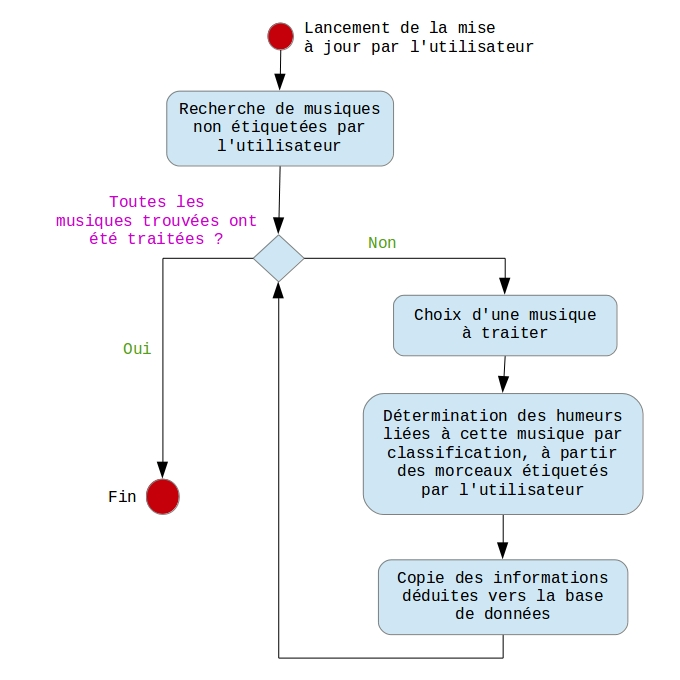
\includegraphics[scale=0.5]{./images/SchemaMiseAJour2.jpg}
\caption{Opérations effectuées lors de le mise à jour de la base de données, avec étiquetage automatique}
\label{ds3}
\end{figure}
		
	\section{Interface utilisateur graphique}
		Le programme, qui sera construit à partir du logiciel libre aTunes, va en reprendre les grandes lignes de l'interface graphique.
On retrouvera donc un découpage en différents panneaux qui permettent à l'utilisateur de naviguer facilement dans sa bibliothèque.

[...]

Une seconde fonctionnalité nécessaire est que l'utilisateur puisse apposer des « tags émotions » à ses différentes musiques.
Ceci serait possible dans le panneau au milieu en haut où s'affiche les chansons en ligne.
Aux colonnes « Titre », « Artiste » et autres on ajouterait alors une colonne « Émotions » qui comprend trois smileys cliquables permettant l'étiquetage des morceaux selon les trois émotions retenues.

Cette colonne ressemblerait dans l'idée à ce qui suit :

\vspace{1em}
\begin{center}\textsf{\begin{tabular}{lcccccc}
	Think		   & \hspace{1cm} \textcolor{Green}{\Smiley}  & \textcolor{Silver}{\Sadey} & \textcolor{Silver}{\Walley} & \textcolor{Silver}{\Neutrey} \\
	\hline
	American Idiot & \hspace{1cm} \textcolor{Silver}{\Smiley} & \textcolor{Silver}{\Sadey} & \textcolor{Silver}{\Walley} & \textcolor{Blue}{\Neutrey} \\
	\hline
	Stone Free	   & \hspace{1cm} \textcolor{Silver}{\Smiley} & \textcolor{Silver}{\Sadey} & \textcolor{Tomato}{\Walley} & \textcolor{Silver}{\Neutrey} \\
	\hline
	L'inverno	   & \hspace{1cm} \textcolor{Silver}{\Smiley} & \textcolor{Red}{\Sadey}    & \textcolor{Silver}{\Walley} & \textcolor{Silver}{\Neutrey} \\
	\hline
	Love Gun	   & \hspace{1cm} \textcolor{Green}{\Smiley}  & \textcolor{Silver}{\Sadey} & \textcolor{Tomato}{\Walley} & \textcolor{Silver}{\Neutrey} \\
	\hline
	Run Rabbit	   & \hspace{1cm} \textcolor{Silver}{\Smiley} & \textcolor{Silver}{\Sadey} & \textcolor{Silver}{\Walley} & \textcolor{Blue}{\Neutrey} \\
\end{tabular}}\end{center}
\vspace{1em}


Enfin la fonction d'étiquetage automatique des chansons non traitées par l'utilisateur serait lancée à partir d'une commande dans le menu « Fichier » à partir duquel on peut déjà demander à l'application de lancer un scan de la bibliothèque pour trouver de nouveaux morceaux.
		
	\section{Tableau détaillé des tâches}
		\begin{tabular}{llm{1.5cm}m{1.5cm}}
	Tâche & Description                                                              & Démontrée au PAN3    & Intégrée au PAN3    \\
	\hline \hline
	T1    & \multicolumn{3}{c}{\cellcolor{LightSteelBlue} Prendre en compte les besoins utilisateur (module Focus Group)}         \\
	T1.1  & Réaliser un guide de discussion                                          &                      & \cs                 \\
	T1.2  & Contacter les participants à la session                                  &                      & \cs                 \\
	T1.3  & Tenir la réunion et filmer, noter, animer, observer                      &                      & \cs                 \\
	T1.4  & Rédiger un rapport sur la réunion                                        &                      & \cs                 \\
	\hline
	T2    & \multicolumn{3}{c}{\cellcolor{LightSteelBlue} Mener une étude de l'impact vie privée de l'application (module Vie privée)}     \\
	T2.1  & Réaliser la première partie du rapport (contextualisation et pertinence) &                      & \cs                 \\
	T2.2  & Réaliser la deuxième partie du rapport sur l'étude des risques           &                      & \cs                 \\
	\hline
	T3    & \multicolumn{3}{c}{\cellcolor{LightSteelBlue} Classifier les images et morceaux par émotions (module classification)} \\
	T3.1  & Réaliser un pseudo-code du classifieur                                   &                      & \cs                 \\
	T3.2  & Implémenter ce code en Java                                              & \cs                  &                     \\
	T3.3  & Valider le classifieur sur des données test                              & \cs                  &                     \\
	T3.4  & Évaluer son efficacité sur nos échantillons (morceaux et images)         & \cs                  &                     \\
	\hline
	T4    & \multicolumn{3}{c}{\cellcolor{LightSteelBlue} Modifier l'interface graphique préexistante (module intégration)}       \\
	T4.1  & Étudier l'interface graphique de aTunes                                  &                      & \cs                 \\
	T4.2  & Réaliser les éléments graphiques (logo, smileys)                         &                      & \cs                 \\
	T4.3  & Intégrer nos créations à l'interface                                     &                      & \cs                 \\
	\hline
	T5    & \multicolumn{3}{c}{\cellcolor{LightSteelBlue} Associer une playlist à une émotion (module recommandation)}            \\
	T5.1  & Définir les paramètres sur lesquels se base la sélection (protocole)     &                      & \cs                 \\
	T5.2  & Coder l'algorithme de constitution de playlist (système fonctionnel)     & \cs                  &                     \\
	\hline
	T6    & \multicolumn{3}{c}{\cellcolor{LightSteelBlue} Création des bases de données (module intégration)}                     \\
	T6.1  & Index des musiques                                                       &                      & \cs                 \\
	T6.2  & Base de données des émotions                                             &                      & \cs                 \\
	T6.3  & Émulation d'une base de musiques en ligne                                & \cs                  &                     \\
	\hline
	T7    & \multicolumn{3}{c}{\cellcolor{LightSteelBlue} Assemblage des différents éléments (module intégration)}                \\
	T7.1  & Étude préalable du code de aTunes                                        &                      & \cs                 \\
	T7.2  & Remplacement de ce qui est modifié par rapport au code d'origine         &                      & \cs                 \\
	T7.3  & Ajout des codes des autres modules pour les fonctionnalités spécifiques  & \cs                  &                     \\
	\hline
	T8    & \multicolumn{3}{c}{\cellcolor{LightSteelBlue} Extraire les données des images (module traitement image)}              \\
	T8.1  & Redressement géométrique d'une image                                     &                      & \cs                 \\
	T8.1  & Transformation RVB/HSV                                                   &                      & \cs                 \\
	T8.1  & Repérage et analyse des composantes connexes                             &                      & \cs                 \\
	T8.1  & Lecture/écriture dans un fichier                                         &                      & \cs                 \\
	T8.1  & Comparaison de deux visages                                              & \cs                  &                     \\
	\hline
	T9    & \multicolumn{3}{c}{\cellcolor{LightSteelBlue} Analyse de caractéristiques audio (module audio MFCC)}                  \\
	T9.1  & Codage et tests de comparaison des MFCC                                  &                      & \cs                 \\
	T9.2  & Intégration avec le module classification                                & \cs                  &
\end{tabular}

\chapter{Organisation du projet}

	\section{Diagramme de planification temporel des tâches}
	Voir figure \ref{gantt}.
	
	\begin{figure}[htp]
		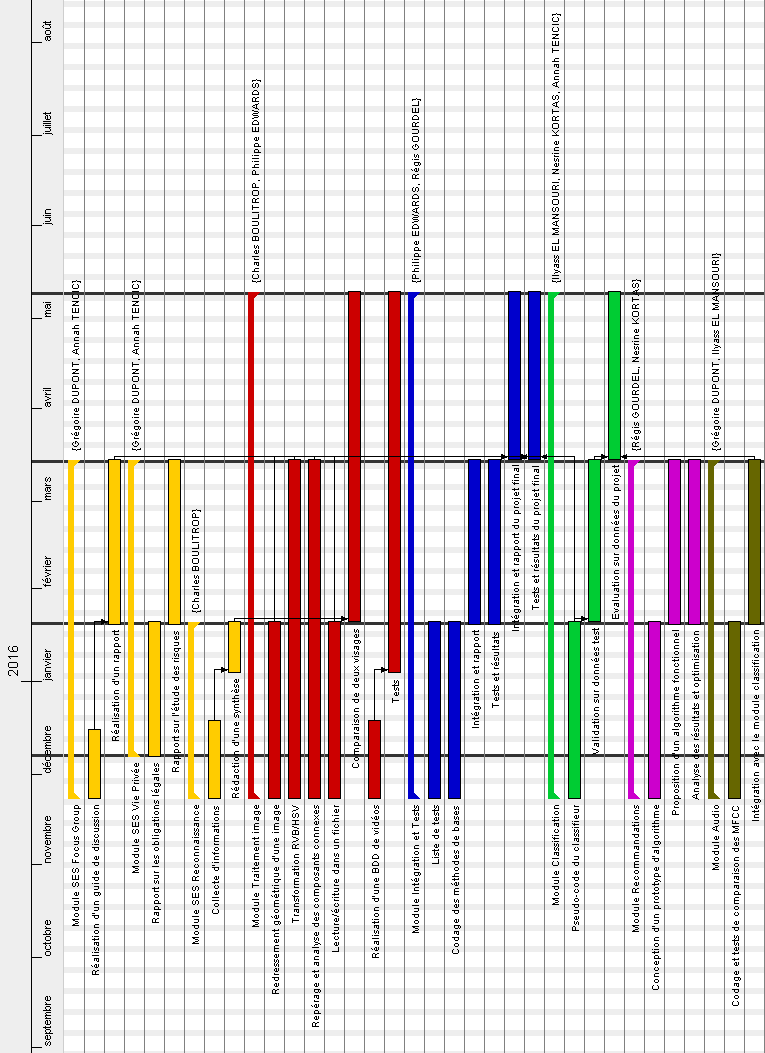
\includegraphics[scale=0.60]{images/gantt2.png}
		\caption{Diagramme chronologique de Gantt}
		\label{gantt}
	\end{figure}
		


\section{Répartition des élèves par module}
	\begin{tabular}{l|l|ccccccc}
		Nom module                   & Nom Expert & A. & N. & G. & I. & P. & C. & R. \\ % Les lettres étaient les initiales de nos prénoms...
		\hline
		Module 1 & Prénom Nom &    &\ct &    &    &    &    &\ct \\
		Module 2 & Prénom Nom &\ct &\ct &    &\ct &    &    &    \\
		Module 3 & Prénom Nom &\ct &    &\ct &    &    &    &    \\
		Module 4 & Prénom Nom &\ct &    &\ct &    &    &    &    \\
		Module 5 & Prénom Nom &    &    &    &    &    &\ct &    \\
		Module 6 & Prénom Nom &    &    &\ct &\ct &    &    &    \\
		Module 7 & Prénom Nom &    &    &    &    &\ct &\ct &    \\
		Module 8 & Prénom Nom &    &    &    &    &\ct &    &\ct
	\end{tabular}


\section{\textcolor{RoyalBlue}{Plans de test}}

	\setlongtables

\begin{longtable}{m{1.9cm}|m{3.9cm}|m{2.9cm}|m{2.9cm}|m{2.5cm}}
	\textbf{Module} & \textbf{Description du test} & \textbf{Entrée} & \textbf{Sortie attendue} & \textbf{Validation} \\
	\hline
	\endhead

	\textcolor{Green}{Image} &
		Test de fonctionnalité : extraction des paramètres en conditions normales &
		Ensemble réduit d'images de visages &
		Paramètres extraits &
		Voir annexe du module \\
	\hline

	\textcolor{Green}{Image} &
		Mesures de performance &
		Une prise (dix images) &
		Temps de calcul de environ 2 s &
		Le temps est satisfaisant.
		Dépend des performances de l'ordinateur. \\
	\hline

	\textcolor{Green}{Classification (images)} &
		Test de fonctionnalité : cas normal avec paramètres choisis &
		Paramètres correspondants à des visages &
		Émotions &
		Taux de succès de 70\% pour un test en validation croisée \\
	\hline

	\textcolor{Green}{Classification (images)} &
		Mesure de performance sur quelques entrées &
		Ensembles de paramètres types correspondants à des visages &
		Temps d'exécution : 1500 ms par prise, variable en fonction des performance de l'appareil. &
		Le temps obtenu est acceptable. \\
	\hline

	\textcolor{Green}{Classification (musiques)} &
		Test de fonctionnalité &
		Plusieurs musiques &
		Émotions associées aux musiques &
		Taux de réussite : 69\%. \\
	\hline

	\textcolor{Green}{Classification (musiques)} &
		Mesure de performance sur quelques entrées &
		Série de 60 musiques. &
		Temps d'exécution : 1500 ms. &
		Le temps est suffisant pour un usage classique, ceci n'étant réalisé que ponctuellement. \\
	\hline

	\textcolor{Green}{Image et classification} &
		Mesure de performance : temps total de reconnaissance de l'émotion &
		Ensembles d'images avec ou sans visage &
		Temps d'exécution 8152 ms &
		Temps acceptable pour cette application. \\
	\hline

	\textcolor{Green}{Audio MFCC} &
		Test de fonctionnalité &
		Ensemble de musiques &
		Moyenne quadratique par rapport à des résultats théorique. &
		Taux d'erreurs : 8\%. \\
	\hline

	\textcolor{Green}{Audio MFCC} &
		Test de performance &
		Ensemble de musiques &
		Temps d'exécution 2000 ms par musique. &
		Valeur un peu trop grande en cas de gros ajout mais passable. \\
	\hline
	
\end{longtable}


\section{Diagramme d’avancement des tâches}

	\subsection{Avancement au PAN 2}
	
	\begin{tabular}{lm{1.9cm}m{1.9cm}m{1.6cm}m{5.1cm}}
		Module & Avancement prévu (\%) & Avancement réel (\%) & Temps passé (h) & Description brève du travail effectué, analyse des écarts constatés \\
		\hline \hline
		Module 1 &
			30\% & 30\% & 18 h &
			Élaboration du plan de test, familiarisation avec le code, compilation et modification de quelques éléments graphiques. \\
		\hline
		Module 2 &
			50\% & 45\% & 20 h &
			Blablabla. \\
		\hline
		Module 3 &
			40\% & 40\% & 10 h &
			Blablabla. \\
		\hline
		Module 4 &
			40\% & 40\% & 10 h &
			Blablabla. \\
		\hline
		Module 5 &
			40\% & 30\% & 20 h &
			Blablabla. \\
		\hline
		Module 6 &
			30\% & 30\% & 20 h &
			Blablabla. \\
		\hline
		Module 7 &
			50\% & 50\% & 5 h &
			Blablabla. \\
		\hline
		Module 8 &
			50\% & 50\% & 3 h &
			Blablabla. \\
		\hline
		Module 9 &
			100\% & 65 \% & 5 h &
			Blablabla.
	\end{tabular}

\subsection{Avancement au PAN 3}

	% Copier-coller le tableau précédent et mettre des avancements plus importants

\subsection{\textcolor{RoyalBlue}{Avancement au PAN 4}}

	% Copier-coller le tableau précédent et mettre des avancements à 100%...


\chapter{Bibliographie}

	\paragraph{Ressources utiles au développement :}

\begin{itemize}
	\item[\textbullet] \bsc{Sourceforge}. \textit{aTunes} [en ligne]. [Consulté le 01/02/2016]. Disponible à l'adresse : \url{http://sourceforge.net/projects/atunes}.
	\item[\textbullet] \bsc{Itseez}. \textit{OpenCV} [en ligne]. [Consulté le 01/02/2016]. Disponible à l'adresse : \url{http://opencv.org}.
\end{itemize}


\paragraph{Documents sur la reconnaissance des émotions}

\begin{itemize}
	\item[\textbullet] \bsc{Clay}, Alexis. \textit{La branche émotion, un modèle conceptuel pour l'intégration de la reconnaissance multimodale d'émotion des application interactives : application au mouvement et à la danse augmentée}. Thèse de doctorat : informatique. Bordeaux : Université Sciences et Technologies - Bordeaux I, 2009.
	\item[\textbullet] \bsc{Hamdi}, Hamza. \textit{Plateforme multimodale pour la reconnaissance d'émotion via l'analyse de signaux physiologiques : Application à la simulation d'entretiens d'embauche} [en ligne]. Thèse de doctorat : informatique. Université d'Angers, 2012. [Consulté le 01/02/2016]. Disponible à l'adresse : \url{https://tel.archives-ouvertes.fr/tel-00997249/document}.
\end{itemize}


\paragraph{Documents pour le traitement audio des musiques}

\begin{itemize}
	\item[\textbullet] \bsc{Davis}, Steven B. et \bsc{Mermelstein}, Paul. Comparison of parametric representations for monosyllabic word recognition in continuously spoken sentences. \textit{Acoustics, Speech and Signal Processing, IEEE Transactions on}, 1980, vol. 28, no 4, p. 357-366.
	\item[\textbullet] \bsc{Huang}, Xuedong, \bsc{Acero}, Alex, \bsc{Hon}, Hsiao-Wuen. \textit{Spoken Language Processing: A Guide to Theory, Algorithm, and System Development} (1st ed.). Prentice Hall PTR, Upper Saddle River, NJ, USA, 2001.
	\item[\textbullet] \bsc{David}, Bertrand. \textit{FPa signal} [en ligne, consulté le 23/02/2016]. Disponible à l'adresse :  \url{http://etenfaitalafin.fr}
	\item[\textbullet] \bsc{Klautau}, Aldebaro. \textit{The MFCC} [en ligne]. 22/11/2005 [consulté le 23/02/2016]. Disponible à l'adresse : \url {http://etenfaitalafin.fr}
	\item[\textbullet] \bsc{Richard}, Gaël, \bsc{Alonso} Miguel. \textit{UE SI350: Travaux pratiques sur l'indexation audio} [en ligne]. Mis à jour le 19/06/2013 [consulté le 23/02/2016]. Disponible à l'adresse : \url{http://etenfaitalafin.fr}
\end{itemize}


\paragraph{Documents pour la recommandation :}

\begin{itemize}
	\item[\textbullet] \bsc{Ji}, Ke, \bsc{Sun}, Runyuan, \bsc{Shu}, Wenhao, et al. Next-song recommendation with temporal dynamics. \textit{Knowledge-Based Systems}, 2015, vol. 88, p. 134-143. doi:\url{http://etenfaitalafin.fr}.
	\item[\textbullet] \bsc{Domingues}, Marcos A. et \bsc{Oliveira Rezende}, Solange. The impact of context-aware recommender systems on music in the long tail. In : \textit{Intelligent Systems (BRACIS), 2013 Brazilian Conference on}. IEEE, 2013. p. 119-124. DOI 10.1109/BRACIS.2013.28.
	\item[\textbullet] \bsc{Takács}, Gábor et \bsc{Tikk}, Domonkos. Alternating least squares for personalized ranking. In : \textit{Proceedings of the sixth ACM conference on Recommender systems}. ACM, 2012. p. 83-90. DOI=\url{http://etenfaitalafin.fr}.
\end{itemize}


\paragraph{Sources pour la classification :}

\begin{itemize}
	\item[\textbullet] \bsc{Ihler}, Alexandre. \textit{Ensembles (4): AdaBoost} [vidéo en ligne]. YouTube, 07/11/2012 [consulté le 23/02/2016]. Disponible à l'adresse : \url{https://youtu.be/dQw4w9WgXcQ}.
\end{itemize}


\paragraph{Documents pour le module image}

\begin{itemize}
	\item[\textbullet] \bsc{Milgram}, Maurice, \bsc{Belaroussi}, Rachid, et \bsc{Prévost}, Lionel. Détection de visages sur des images fixes par combinaison de classifieurs discriminants et de modèles. In : \textit{19° Colloque sur le traitement du signal et des images, FRA, 2003}. GRETSI, Groupe d’Etudes du Traitement du Signal et des Images, 2003. Disponible à l'adresse : \url{http://xkcd.com/1608/}.
	\item[\textbullet] \bsc{Le Martelot}, Erwan. \textit{Détection de Visages à l’Aide de Réseaux de Neurones} [en ligne]. 17/01/2005 [consulté le 23/02/2016]. Disponible à l'adresse : \url{http://endless.horse/}.
\end{itemize}


%%%%%%%%%%%%%%%%%%%%%
% Début des annexes %
%%%%%%%%%%%%%%%%%%%%%

\appendix

\chapter{Fiche d'identité de groupe}
	\section{Présentation collective}

	Blablabla

\section{Présentation des membres du groupe}

	\subsection{Étudiant 1}
		\paragraph*{Parcours}
			Blablabla
		\paragraph*{Points forts}
			Blablabla
		\paragraph*{Craintes}
			Blablabla
	
	\subsection{Étudiant 2}
		Blablabla
	
	\subsection{Étudiant 3}
		\paragraph*{Parcours}
			Blablabla
		\paragraph*{Points forts}
			Blablabla
		\paragraph*{Points faibles}
			Blablabla
		\paragraph*{Intérêts}
			Blablabla
	
	\subsection{Étudiant 4}
		\paragraph*{Parcours}
			Blablabla
		\paragraph*{Points forts}
			Blablabla
		\paragraph*{Points faibles et craintes}
			Blablabla
		\paragraph*{Intérêts}
			Blablabla	
	
	\subsection{Étudiant 5}
		\paragraph*{Parcours}
			Blablabla
		\paragraph*{Points forts}
			Blablabla
		\paragraph*{Points faibles}
			Blablabla	
	
	\subsection{Étudiant 6}
		\paragraph*{Parcours}
			Blablabla
		\paragraph*{Points forts}
			Blablabla
		\paragraph*{Points faibles}
			Blablabla
		\paragraph*{Craintes}
			Blablabla
		\paragraph*{Intérêt}
			Blablabla	
	
	\subsection{Étudiant 7}
		\paragraph*{Mensurations}
			Blablabla 1m75, 83C, 62, 85
		\paragraph*{Score au test de Griffor}
			Blablabla 105
		\paragraph*{Film préféré}
			Blablabla Le triomphe de Babar


\chapter{Compte-rendus de réunions}
	\section{Descriptif chronologique des réunions}

	Les rendez-vous avec experts par modules ne sont pas répertoriés.

	Légende :
	\begin{itemize}
		\item \textcolor{Blue}{séance encadrée prévue dans l'emploi du temps}
		\item \textcolor{Purple}{séance en autonomie prévue dans l'emploi du temps}
		\item \textcolor{Green}{réunion non prévue dans l'emplois du temps mais encadrée}
		\item \textcolor{Red}{réunion non prévues dans l'emploi du temps en autonomie}
	\end{itemize}

	\begin{description}
		\item[\textcolor{Blue}{29.09.15}]
			Premier contact tuteurs : team building ( réalisation de tours en papier) et recherche d'idées de sujets pour les 2 thèmes PACT annoncés (CR en \ref{CR1}).
		\item[\textcolor{Red}{01.10.15}]
			Choix parmi 14 de 3 sujets : Jogging, SmartMouth et Délécom retenus.
		\item[\textcolor{Blue}{05.10.15}]
			Remise en question du sujet jogging, remplacé par le sujet Feux de Forêts.\\
			Présentation des sujets à l'instar d'une start-up cherchant des clients et des fonds, questions entre membres du groupe.\\
			1er tri des cartes modules.
		\item[\textcolor{Red}{07.10.15}]
			Discussion sur les détails des 3 projets retenus.\\
			Répartition du travail pour les posters et brouillons des posters pour la foire aux experts.
		\item[\textcolor{Blue}{12.10.15}]
			Foire aux experts : SmartMouth et 3Délécom abandonnés, nouvelle idée FeelList et Feux de forêts réalisable mais moins attrayant (CR en \ref{CR2}).
		\item[\textcolor{Blue}{14.10.15}]
			Foire aux modules puis débrief sur la foire aux experts avec tuteurs (un compte-rendu individuel effectué par présentation, voir \ref{CR3.1} à \ref{CR3.5}).
		\item[\textcolor{Red}{16.10.15}]
			Discussion du détail des 2 sujets encore en lice (FeelList et Feux de forêts).\\
			Classement des cartes modules.
		\item[\textcolor{Blue}{19.10.15}]
			Pour choisir entre FeelList et Feux de forêts tous les memebres qui aiment le moins un sujet doivent défendre ses avantages.\\
			Commencement de répartition des modules au tableau.\\
			Explications relatives au scénario utilisateur SES à rédiger pendant les vacances.
		\item[\textcolor{Red}{23.10.15}]
			Discussion détaillée sur FeelList (sujet principal).\\
			Scénario de secours Feux de forêts.\\
			(CR en \ref{CR4.1}, \ref{CR4.2} et \ref{CR4.3})
		\item[\textcolor{Blue}{05.11.15}]
			Scénario corrigé par experte ses, et modifications pour tenir compte de ses conseils.
		\item[\textcolor{Blue}{09.11.15}]
			Foire libre : mini-cours de classification et rendez-vous SES.
		\item[\textcolor{Red}{25.10.15 au soir}]
			Réunion pour prendre en compte les remarques faites au cours du rendez-vous SES.
		\item[\textcolor{Green}{13.11.15}]
			Point avec tuteurs (rapport PAN 1, contrats avec experts).\\
			Répartition des modules entre nous.\\
			(CR en \ref{CR6})
		\item[\textcolor{Blue}{16.11.15}]
			Cours de l'expert GL (présentation des diagrammes d'architecture et d'activité).
		\item[\textcolor{Purple}{17.11.15}]
			Réalisation des diagrammes.
			Envoi de mails aux experts pour prise de rendez-vous modules.
		\item[\textcolor{Red}{20.11.15}]
			Détails supplémentaires quant au fonctionnement de FeelList, au rôle exact de chaque module, à la prise de contacts avec experts, aux questions subsistant (CR en \ref{CR7}).
		\item[\textcolor{Blue}{24.11.15}]
			Séance avec l'expert GL : correction des diagrammes et création d'un dépôt git pour notre groupe.
		\item[\textcolor{Purple}{25.11.15}]
			Préparation du PAN 1 : répartition des tâches.\\
			Rendez-vous experts.\\
			(CR en \ref{CR8})
		\item[\textcolor{Red}{30.11.15}]
			Touches finales du rapport PAN 1.\\
			Préparation de l'intervention orale PAN 1.
		\item[\textcolor{Blue}{08.12.15}]
			Réunion avec tuteurs pour faire le point sur le PAN 1 et discuter de l'avancement jusqu'au PAN 2.
		\item[\textcolor{Red}{14.12.15}]
			Point en autonomie du groupe.
		\item[\textcolor{Blue}{15.12.15}]
			Plans de test avec l'expert GL.
		\item[\textcolor{Red}{04.01.16}]
			Point en autonomie pour organiser le focus group.
		\item[\textcolor{Red}{11.01.16}]
			Point en autonomie en prévision du PAN 2, distribution des tâches, organisation du rapport écrit et de la soutenance orale.
	\end{description}


\section{Compte-rendu du xx.xx.16 : 1\up{er} contact tuteurs}
	\label{CR1}


\section{Compte-rendu du 12.10.15 : Foire aux experts}
	\label{CR2}


\section{CR foire aux modules : SES}
	\label{CR3.1}


\section{CR foire aux modules : Electronique}
	\label{CR3.2}

% ...

% Modules
% Pensez à changer les noms dans les titres...
\chapter{Module 1}
	\section{Fiche module}
	\noindent Nom du module : \textbf{le nom du module}.\\
	Encadrant : \textbf{Prénom Nom}. \\

	GROUPE X.X
	Élèves : \textbf{Prénom \textsc{Nom}} et \textbf{Prénom \textsc{Nom}}.

\section{Documentation}

	\begin{itemize}
	\item[\textbullet] un bouqiuin utile
	\item[\textbullet] une thèse sympa
	\item[\textbullet] \url {un truc en ligne}
	\end{itemize}

\section{Avancement} % Pour les PANs > 1, la structure est juste une suggestion

	\paragraph*{Avancées au PAN n-1.}
	pipo

	\paragraph*{\textcolor{RoyalBlue}{Avancées au PAN n.}}
	pipo

	\paragraph*{Difficultés.}
	on est un peu nuls.

\chapter{Module 2}
	\section{Fiche module}
	\noindent Nom du module : \textbf{le nom du module}.\\
	Encadrant : \textbf{Prénom Nom}. \\

	GROUPE X.X
	Élèves : \textbf{Prénom \textsc{Nom}} et \textbf{Prénom \textsc{Nom}}.

\section{Documentation}

	\begin{itemize}
	\item[\textbullet] un bouqiuin utile
	\item[\textbullet] une thèse sympa
	\item[\textbullet] \url {un truc en ligne}
	\end{itemize}

\section{Avancement} % Pour les PANs > 1, la structure est juste une suggestion

	\paragraph*{Avancées au PAN n-1.}
	pipo

	\paragraph*{\textcolor{RoyalBlue}{Avancées au PAN n.}}
	pipo

	\paragraph*{Difficultés.}
	on est un peu nuls.

\chapter{Module 3}
	\section{Fiche module}
	\noindent Nom du module : \textbf{le nom du module}.\\
	Encadrant : \textbf{Prénom Nom}. \\

	GROUPE X.X
	Élèves : \textbf{Prénom \textsc{Nom}} et \textbf{Prénom \textsc{Nom}}.

\section{Documentation}

	\begin{itemize}
	\item[\textbullet] un bouqiuin utile
	\item[\textbullet] une thèse sympa
	\item[\textbullet] \url {un truc en ligne}
	\end{itemize}

\section{Avancement} % Pour les PANs > 1, la structure est juste une suggestion

	\paragraph*{Avancées au PAN n-1.}
	pipo

	\paragraph*{\textcolor{RoyalBlue}{Avancées au PAN n.}}
	pipo

	\paragraph*{Difficultés.}
	on est un peu nuls.

\chapter{Module 4}
	\section{Fiche module}
	\noindent Nom du module : \textbf{le nom du module}.\\
	Encadrant : \textbf{Prénom Nom}. \\

	GROUPE X.X
	Élèves : \textbf{Prénom \textsc{Nom}} et \textbf{Prénom \textsc{Nom}}.

\section{Documentation}

	\begin{itemize}
	\item[\textbullet] un bouqiuin utile
	\item[\textbullet] une thèse sympa
	\item[\textbullet] \url {un truc en ligne}
	\end{itemize}

\section{Avancement} % Pour les PANs > 1, la structure est juste une suggestion

	\paragraph*{Avancées au PAN n-1.}
	pipo

	\paragraph*{\textcolor{RoyalBlue}{Avancées au PAN n.}}
	pipo

	\paragraph*{Difficultés.}
	on est un peu nuls.

\chapter{Module 5}
	\section{Fiche module}
	\noindent Nom du module : \textbf{le nom du module}.\\
	Encadrant : \textbf{Prénom Nom}. \\

	GROUPE X.X
	Élèves : \textbf{Prénom \textsc{Nom}} et \textbf{Prénom \textsc{Nom}}.

\section{Documentation}

	\begin{itemize}
	\item[\textbullet] un bouqiuin utile
	\item[\textbullet] une thèse sympa
	\item[\textbullet] \url {un truc en ligne}
	\end{itemize}

\section{Avancement} % Pour les PANs > 1, la structure est juste une suggestion

	\paragraph*{Avancées au PAN n-1.}
	pipo

	\paragraph*{\textcolor{RoyalBlue}{Avancées au PAN n.}}
	pipo

	\paragraph*{Difficultés.}
	on est un peu nuls.

\chapter{Module 6}
	\section{Fiche module}
	\noindent Nom du module : \textbf{le nom du module}.\\
	Encadrant : \textbf{Prénom Nom}. \\

	GROUPE X.X
	Élèves : \textbf{Prénom \textsc{Nom}} et \textbf{Prénom \textsc{Nom}}.

\section{Documentation}

	\begin{itemize}
	\item[\textbullet] un bouqiuin utile
	\item[\textbullet] une thèse sympa
	\item[\textbullet] \url {un truc en ligne}
	\end{itemize}

\section{Avancement} % Pour les PANs > 1, la structure est juste une suggestion

	\paragraph*{Avancées au PAN n-1.}
	pipo

	\paragraph*{\textcolor{RoyalBlue}{Avancées au PAN n.}}
	pipo

	\paragraph*{Difficultés.}
	on est un peu nuls.

\chapter{Module 7}
	\section{Fiche module}
	\noindent Nom du module : \textbf{le nom du module}.\\
	Encadrant : \textbf{Prénom Nom}. \\

	GROUPE X.X
	Élèves : \textbf{Prénom \textsc{Nom}} et \textbf{Prénom \textsc{Nom}}.

\section{Documentation}

	\begin{itemize}
	\item[\textbullet] un bouqiuin utile
	\item[\textbullet] une thèse sympa
	\item[\textbullet] \url {un truc en ligne}
	\end{itemize}

\section{Avancement} % Pour les PANs > 1, la structure est juste une suggestion

	\paragraph*{Avancées au PAN n-1.}
	pipo

	\paragraph*{\textcolor{RoyalBlue}{Avancées au PAN n.}}
	pipo

	\paragraph*{Difficultés.}
	on est un peu nuls.

\chapter{Module 8}
	\section{Fiche module}
	\noindent Nom du module : \textbf{le nom du module}.\\
	Encadrant : \textbf{Prénom Nom}. \\

	GROUPE X.X
	Élèves : \textbf{Prénom \textsc{Nom}} et \textbf{Prénom \textsc{Nom}}.

\section{Documentation}

	\begin{itemize}
	\item[\textbullet] un bouqiuin utile
	\item[\textbullet] une thèse sympa
	\item[\textbullet] \url {un truc en ligne}
	\end{itemize}

\section{Avancement} % Pour les PANs > 1, la structure est juste une suggestion

	\paragraph*{Avancées au PAN n-1.}
	pipo

	\paragraph*{\textcolor{RoyalBlue}{Avancées au PAN n.}}
	pipo

	\paragraph*{Difficultés.}
	on est un peu nuls.

\chapter{Module 9}
	\section{Fiche module}
	\noindent Nom du module : \textbf{le nom du module}.\\
	Encadrant : \textbf{Prénom Nom}. \\

	GROUPE X.X
	Élèves : \textbf{Prénom \textsc{Nom}} et \textbf{Prénom \textsc{Nom}}.

\section{Documentation}

	\begin{itemize}
	\item[\textbullet] un bouqiuin utile
	\item[\textbullet] une thèse sympa
	\item[\textbullet] \url {un truc en ligne}
	\end{itemize}

\section{Avancement} % Pour les PANs > 1, la structure est juste une suggestion

	\paragraph*{Avancées au PAN n-1.}
	pipo

	\paragraph*{\textcolor{RoyalBlue}{Avancées au PAN n.}}
	pipo

	\paragraph*{Difficultés.}
	on est un peu nuls.

\end{document}
